\section{Materials}

\begin{itemize}
    \item At least one light curve for each planet of interest. Pre-prepared light curves were downloaded from the NASA Exoplanet Archive, but could
        also be generated from telescope imagery. \autocite{exoplanetArchive}
    \item Software to analyze the light curves. The implementation developed for this experiment has been published on \href{https://github.com/roguePanda/exoplanet-project}{GitHub}.
\end{itemize}

\section{Set-Up}

Since the data for this experiment came from the Kepler mission, a brief overview of the Kepler satellite and processing pipeline will be given.
The Kepler mission was designed to survey a fixed region of the galaxy for several years to detect Earth-sized exoplanets using the transit method. \autocite{keplerManual}
The satellite's sole instrument is a photometer consisting of a CCD array, from which pixels are combined into 30-minute long cadence data and
1-minute short cadence data. \autocite{keplerManual} Once downloaded, the data are calibrated and converted into light curves and target pixel files \autocite{keplerManual}.
The data is eventually made available to the public after a few months. Some of the data presented in this paper were obtained from the Multimission
Archive at the Space Telescope Science Institute (MAST). STScI is operated by the Association of Universities for Research in Astronomy, Inc., under NASA contract NAS5-26555.
Support for MAST for non-HST data is provided by the NASA Office of Space Science via grant NAG5-7584 and by other grants and contracts.
% That last bit is required by the MAST people

\begin{figure}[H]
    \centering
    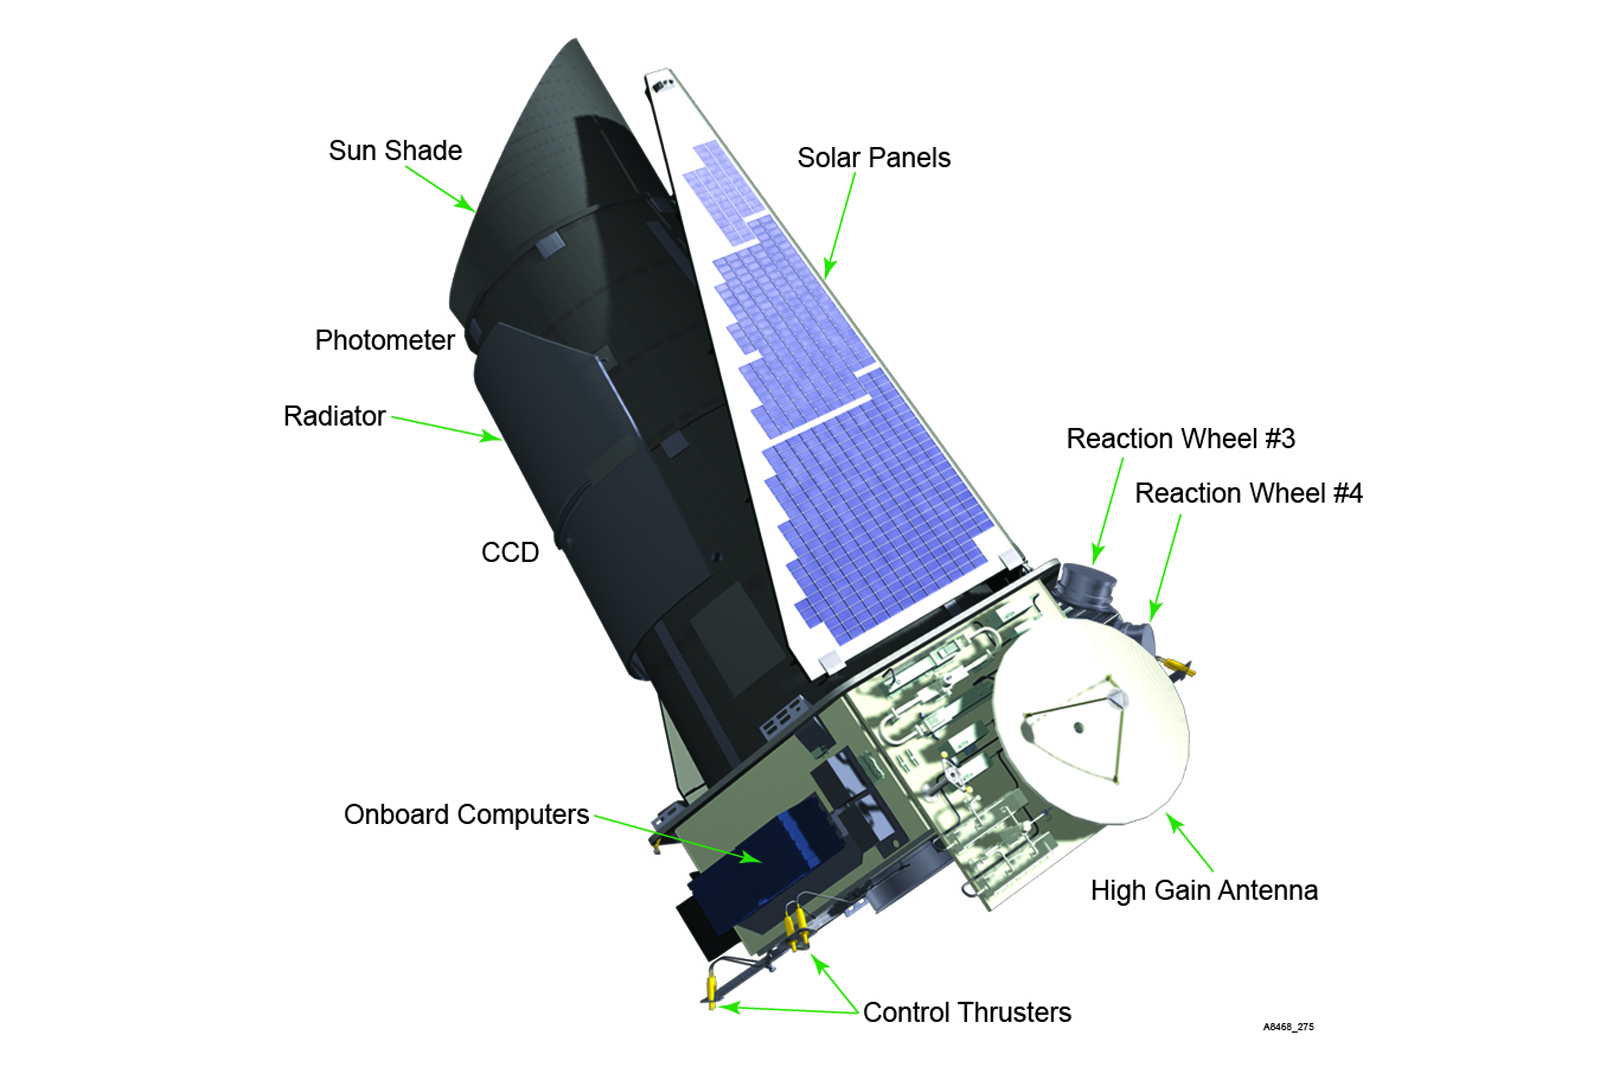
\includegraphics[width=0.6\textwidth]{images/750603main_Ball_Kepler_A8468_275_lg}
    \caption{The Kepler Satellite \autocite{keplerReactionWheelUpdate}}
\end{figure}

\section{Procedure}

\begin{enumerate}
    \item Light curves for Kepler-6b and Kepler-12b were obtained from the \href{http://exoplanetarchive.ipac.caltech.edu/}{NASA Exoplanet Archive}.
    \item The light curves were cleaned by removing all non-finite data points.
    \item The flux in each light curve was normalized by dividing by the median to aid in detrending and periodogram generation.
    \item The light curves were detrended by using least-squares regression to remove global trends. \autocite{untrendy}
    \item A periodogram of each light curve was generated using the box-fitting least squares algorithm. \autocite{bls, pythonBls}
    \item The periodogram and light curve were plotted so that transits and periods could be observed.
    \item The best period was determined from the periodogram by locating the highest peak.
    \item The transit epoch, ingresses, and egresses were determined from the light curve and period.
    \item The transit depth was calculated using the calculated list of transits.
    \item The estimated planetary radius was calculated from the transit depth and the stellar radius as listed in the Extrasolar Planets Encyclopedia. \autocite{exoplanetEncyclopedia}
    \item The percent errors between observed and actual values of the radius and period were calculated.
\end{enumerate}
